% A simple equation for modeling population growth is the exponential ordinary differential equation (ODE), displayed below~\cite{tsoularis2002analysis},
% \begin{equation}\label{eq:expgrowthODE}
%     \frac{dx}{dt} = rx, \quad \text{where}\quad x(0) = x_0.
% \end{equation}
% Consider $r= \text{Birth} - \text{Death}>0$, then $r$ is a constant representing the growth rate of the population at any given time.
% Also, $x$ is the population at time $t$, so $\displaystyle \frac{dx}{dt}$ is the population rate of change that is dependent on $t$.
% As $t$ increases to infinity, the population, $x$, will also approach infinity due to the growth being exponential.
% So, a more accurate way to describe population growth is using a logistic growth ODE, which is given below~\cite{tsoularis2002analysis},
% \begin{equation}\label{eq:logisticgrowthODE}
%     \frac{dx}{dt} = rx\left(1-\frac{x}{K}\right).
% \end{equation}
% Here, $r$ still represents the growth rate of the population, and $K$ serves as the carrying capacity.
% Most species follow a logistic growth pattern due to environmental constraints, such as location, food, and other essential resources. 
% A great way to visualize $K$ as a carrying capacity is by graphing the right-hand side of~\equationautorefname \eqref{eq:logisticgrowthODE} as a function of $x$.
% \begin{figure}[H]
%     \centering
%     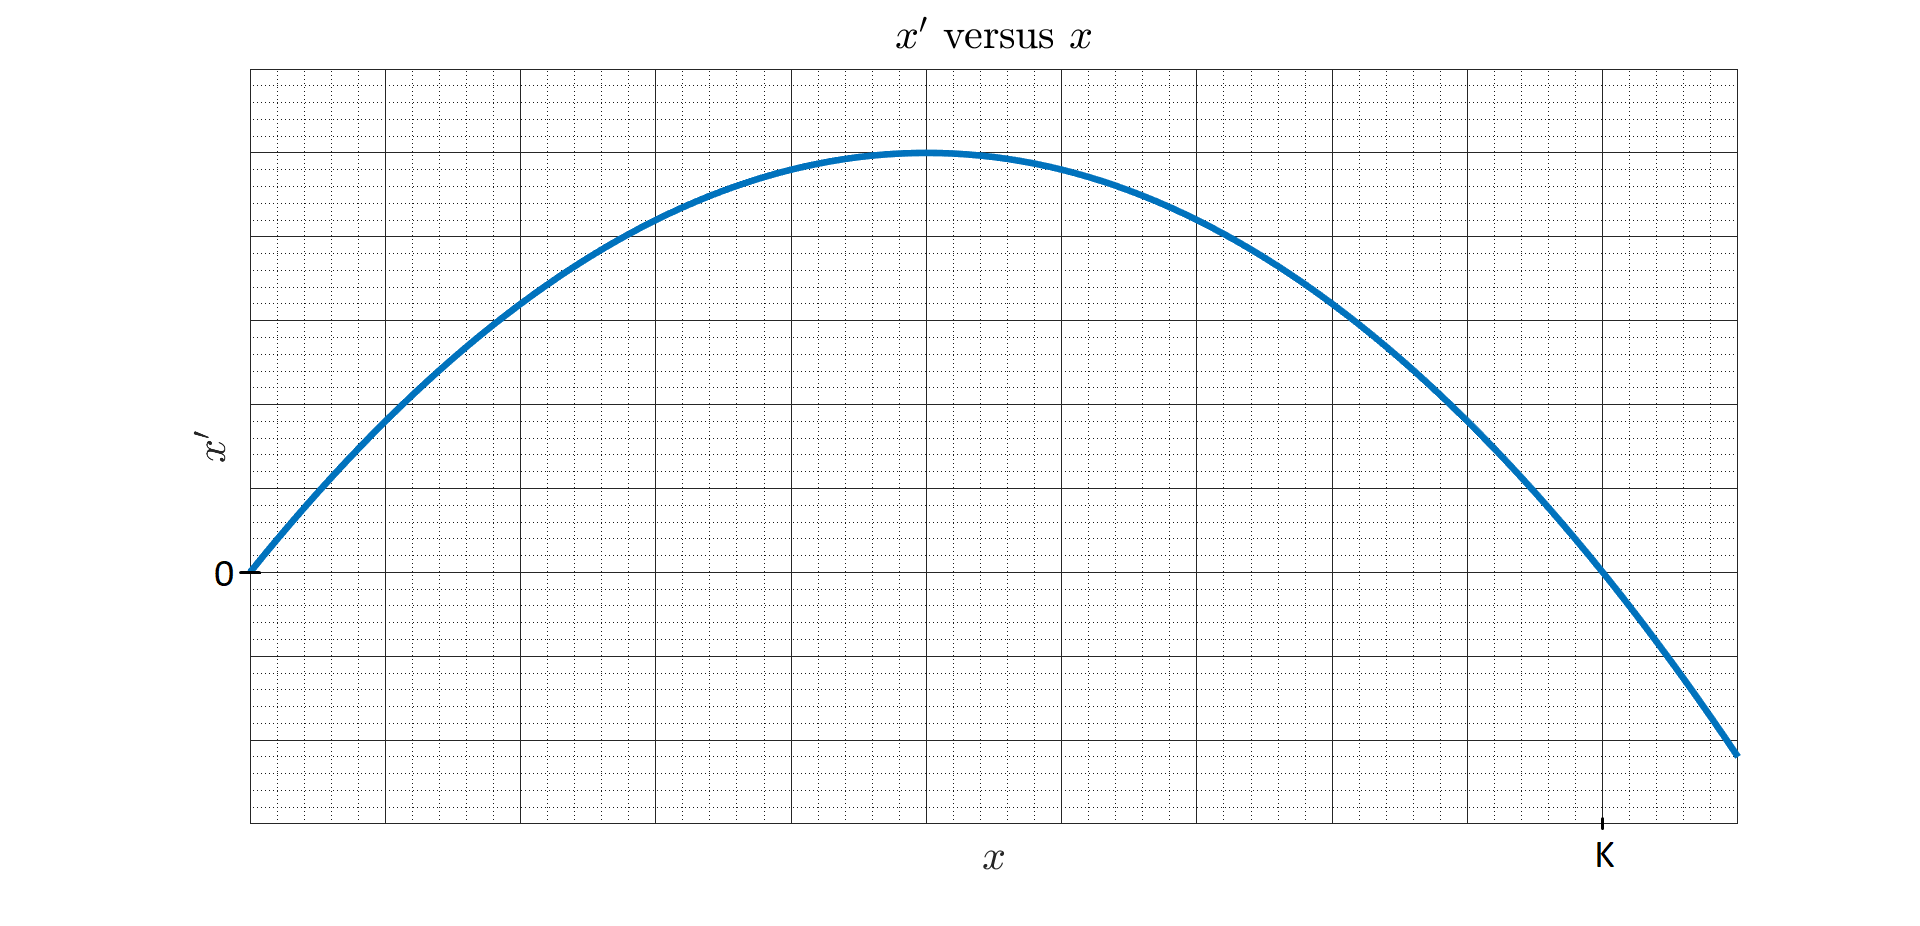
\includegraphics[width=14cm]{Pictures/ODE/LogODE.png}
%     \caption{Plot of the logistic growth equation as a function of $x$.}
%     \label{fig:logisticgrowthODE}
% \end{figure}
% The figure above illustrates that the population, $x$, will continue to grow when $x<K$, but decrease when $x>K$. The population will always be converging towards $K$, which is what we would expect to see in the real world. Thus, the logistic model is a more accurate representation of a specie's population.

% % by using the Lotka-Volterra equation an interaction between two species can be modeled.